\clearpage
\twocolumn[{%
\rqparent
\subsection{English-only models}
\label{app:rq13_english_only}

\noindent\begin{minipage}[t]{0.485\textwidth}
\vspace{0pt}
\paragraph{Research Question.} \emph{The English-only cells (K = 1) train on English alone, while every other cell gives English half of its tokens. Do they score better on the English benchmarks than multilingual cells of the same size? If the runs are correct, they should score higher, clear chance at a smaller size, and be at least as predictable across sizes, as reliable in their decisions (decision accuracy) and as high in SNR. Do their numbers also land where AllenAI's DataDecide puts the same English tasks?}

\paragraph{Setup.} We measure, in accuracy points above chance, how much better a model trained on English alone scores on English benchmarks than one that gives English half of its tokens. We compare the English-only cells (K = 1) with the baseline cells (scheme A, T = 1) of the same depth at every other language setting: deep against deep and shallow against shallow. All cells use seed 1904 and their final checkpoints, 90M--1.7B. We use the English accuracy tasks that are above chance at each size, so the task set changes with the size. For each size, task and language setting, we subtract the multilingual cell's score from the English-only cell's, then average over the tasks and count the share of (task, K) comparisons where the English-only cell is ahead. We also draw the scaling regimes of the English tasks (whether a task scales predictably across sizes, along training, both or neither) for the English-only cell of each English corpus (Figure~\ref{fig:app_rq13_english_scaling_regimes}), and the same regimes on the English accuracy tasks alone (Figures~\ref{fig:app_rq13_english_scaling_regimes_l1_accuracy} and~\ref{fig:app_rq13_english_scaling_regimes_l1_accuracy_tagged}).
\end{minipage}\hfill
\begin{minipage}[t]{0.485\textwidth}
\vspace{0pt}
\begin{rqfinding}
\textbf{1. The English-only cells are better at English, but only by about one accuracy point at 1.7B.} Deep K1 wins more than half of the English accuracy tasks against every other K at every drawn size (25 of 25 (size, K) cells), and its mean gap at 1.7B is 1.1 points over 40 tasks. (Figure~\ref{fig:app_rq13_english_only}.)
\\
\\
\textbf{2. K1 has the lower English BPB in every comparison.} Its \texttt{bpb\_dclm} is lower in all 30 (size, K) comparisons at both depths, and the deep gap shrinks from 0.049 bits per byte at 90M to 0.028 at 1.7B (0.782 against 0.810).
\\
\\
\textbf{3. Part of the lead is larger than the seed noise.} Deep K1 is ahead by more than two seed standard deviations (sd) in 0.50 (175M), 0.43 (600M) and 0.47 (1B) of the (task, K) comparisons, and behind by as much in only 0.03--0.07.
\end{rqfinding}
\end{minipage}

\vspace{\baselineskip}
\noindent\begin{minipage}{\textwidth}
\centering
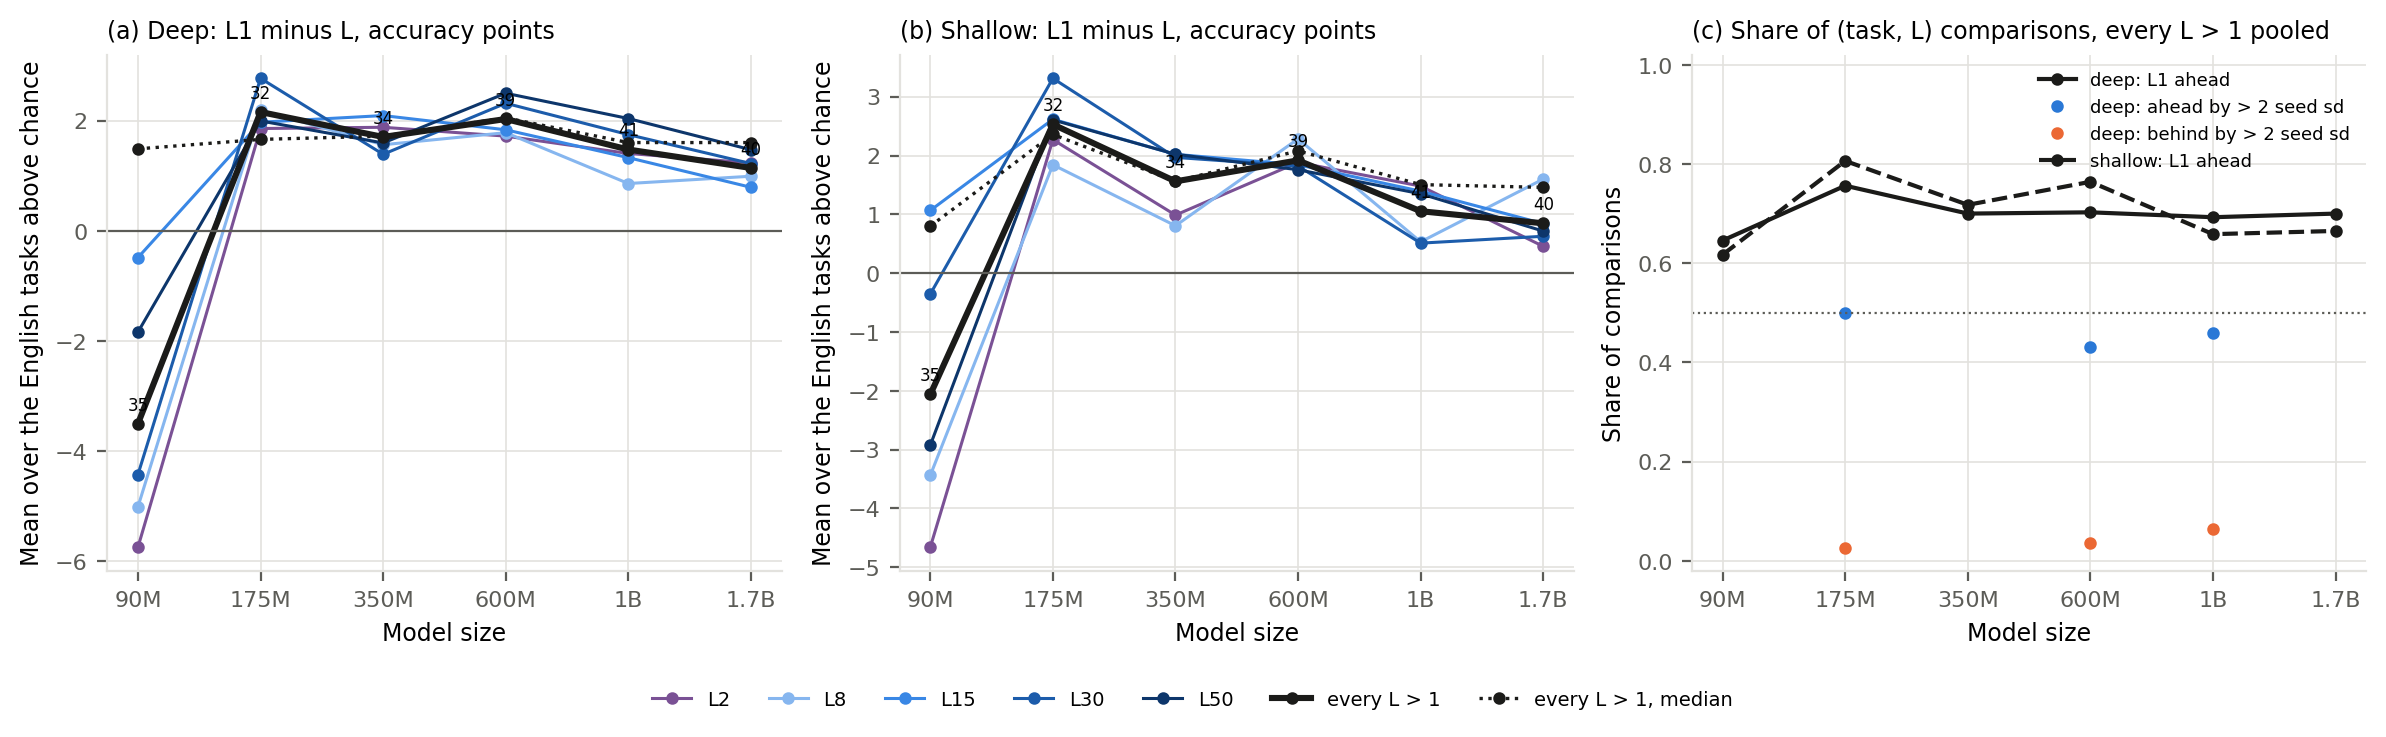
\includegraphics[width=\textwidth,height=0.36\textheight,keepaspectratio]{figures/app_rq13_english_only.png}
% source: src/signal-and-noise/analysis/rq13_english_only/pretraining/predictivity/english_only_scores_paper.png
\captionof{figure}{\textbf{The English-only cells are better at English, but only by about one accuracy point at 1.7B.} (a) and (b): the English-only cells (K = 1) minus the cells with K $>$ 1 of the same size, in accuracy points above chance averaged over the English tasks above chance, for the deep and the shallow ladder. There is one line per K, the thick line pools every K $>$ 1 and the dotted line is their median. (c): the share of (task, K) comparisons in which the English-only cell is ahead.}
\label{fig:app_rq13_english_only}
\end{minipage}
}]

\begin{figure*}[p]
\centering
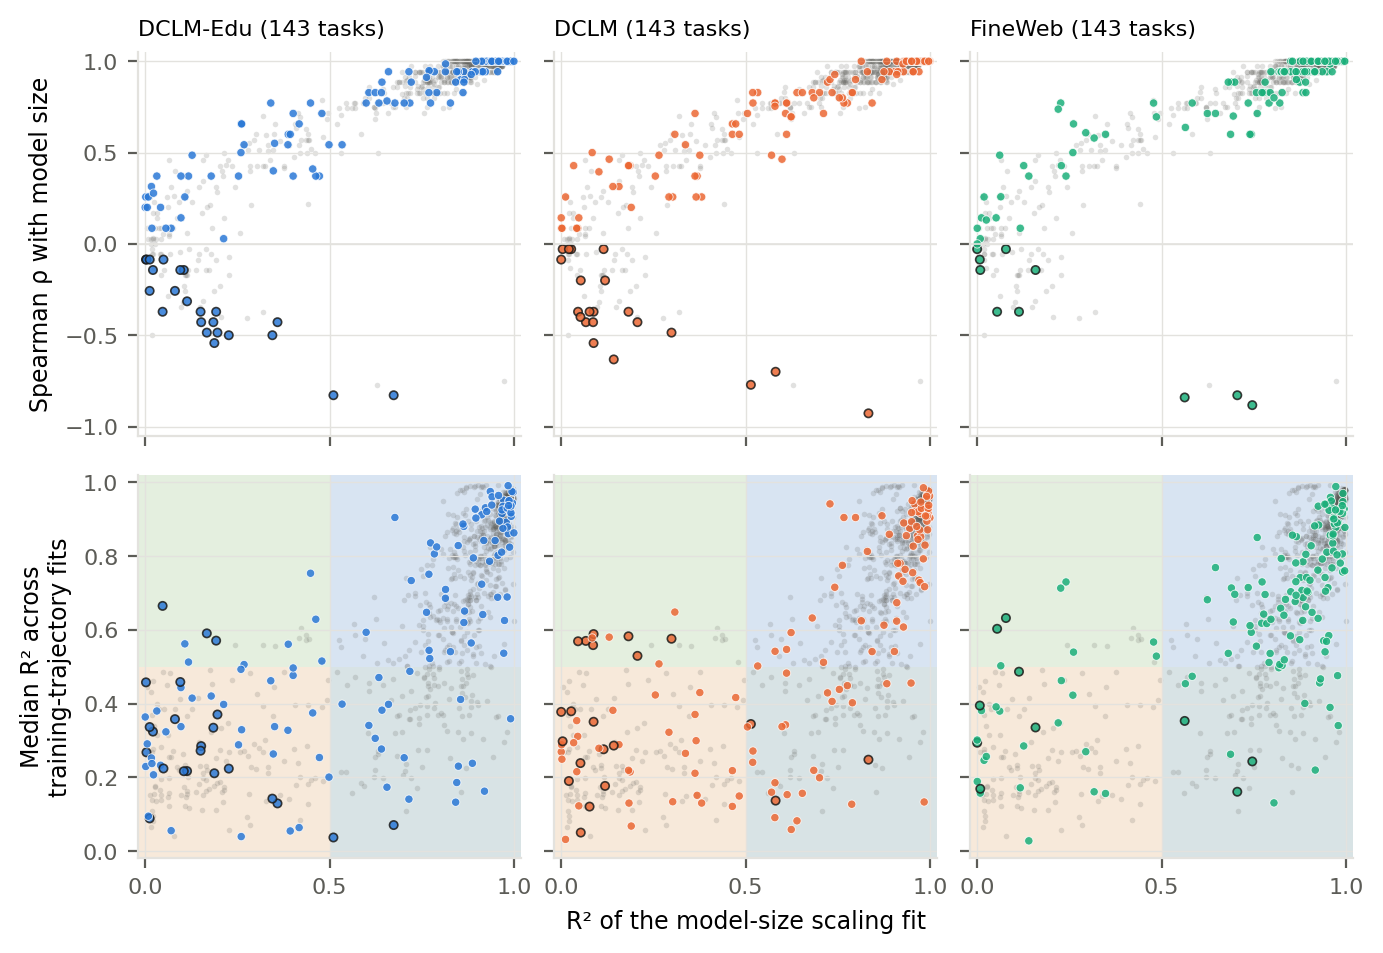
\includegraphics[width=\textwidth,height=0.8\textheight,keepaspectratio]{figures/app_rq13_english_scaling_regimes.png}
% source: src/signal-and-noise/analysis/rq13_english_only/pretraining/predictivity/english_only_scaling_regimes_paper.png
\caption{\textbf{At $K$ = 1 the FineWeb cell puts 69\% of the English tasks in the regime predictable across both size and training, against 45\%--45\% for the two DCLM corpora.} The scaling regimes of Figure~\ref{fig:rq1} drawn for the monolingual English cells, one column per English corpus: DCLM-Edu (the English of every other cell), DCLM without the educational filter, and FineWeb. Each is one deep cell at seed 1904, 90M--1.7B, on the same 143 English tasks (originals, RF, LLM-RF, bBPB twins and the English bits per byte). The FineWeb lead comes from the bBPB twins. On the 39 accuracy tasks alone, the three corpora reach 54\% (DCLM-Edu), 54\% (DCLM), 49\% (FineWeb). The fits and the above-chance gate are those of Figure~\ref{fig:rq1}. With one $K$, a task has one model-size fit instead of a median over the six $K$, and the trajectory $R^2$ is the median over at least two sizes. Top: the $R^2$ of the model-size fit against its Spearman $\rho$. Bottom: the same $R^2$ against the median $R^2$ of the training-trajectory fits, shaded by regime at 0.5. A black edge marks a task whose score declines with size. The grey points are the 1107 tasks of Figure~\ref{fig:rq1} (medians over $K$, 78\% predictable across both), so they sit higher than a single fit would.}
\label{fig:app_rq13_english_scaling_regimes}
\end{figure*}

\begin{figure*}[p]
\centering
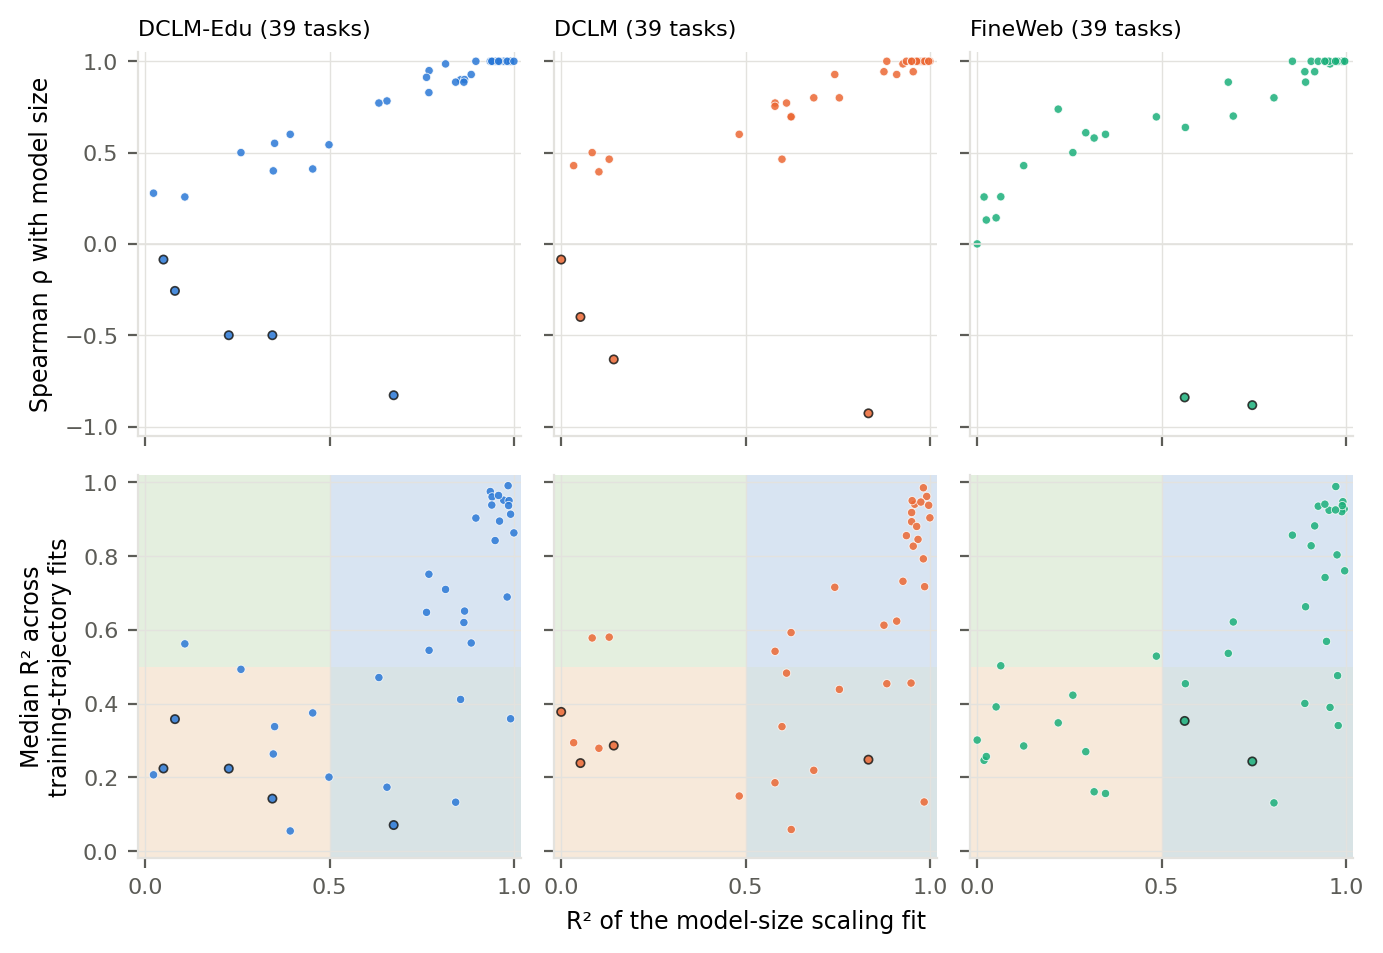
\includegraphics[width=\textwidth,height=0.8\textheight,keepaspectratio]{figures/app_rq13_english_scaling_regimes_l1_accuracy.png}
% source: src/signal-and-noise/analysis/rq13_english_only/pretraining/predictivity/english_only_scaling_regimes_l1_accuracy_paper.png
\caption{\textbf{On the English benchmarks alone, the three English corpora put 49\%--54\% of the tasks in the regime predictable across both size and training, so the FineWeb lead of Figure~\ref{fig:app_rq13_english_scaling_regimes} comes from the bBPB twins.} The same scaling regimes restricted to the monolingual English cells ($K$ = 1) and the English benchmarks. Each column is one deep cell at seed 1904, 90M--1.7B, on the same 39 English accuracy tasks (18 originals, 20 RF and 1 LLM-RF). The bBPB twins, the English bits per byte and every cell with $K > 1$ are left out, so no point comes from a multilingual model. The fits and the above-chance gate are those of Figure~\ref{fig:rq1}. Per corpus, 67\%--83\% of the originals and 25\%--30\% of the RF twins are predictable across both. Top: the $R^2$ of the model-size fit against its Spearman $\rho$. Bottom: the same $R^2$ against the median $R^2$ of the training-trajectory fits, shaded by regime at 0.5. A black edge marks a task whose score declines with size.}
\label{fig:app_rq13_english_scaling_regimes_l1_accuracy}
\end{figure*}

\begin{figure*}[p]
\centering
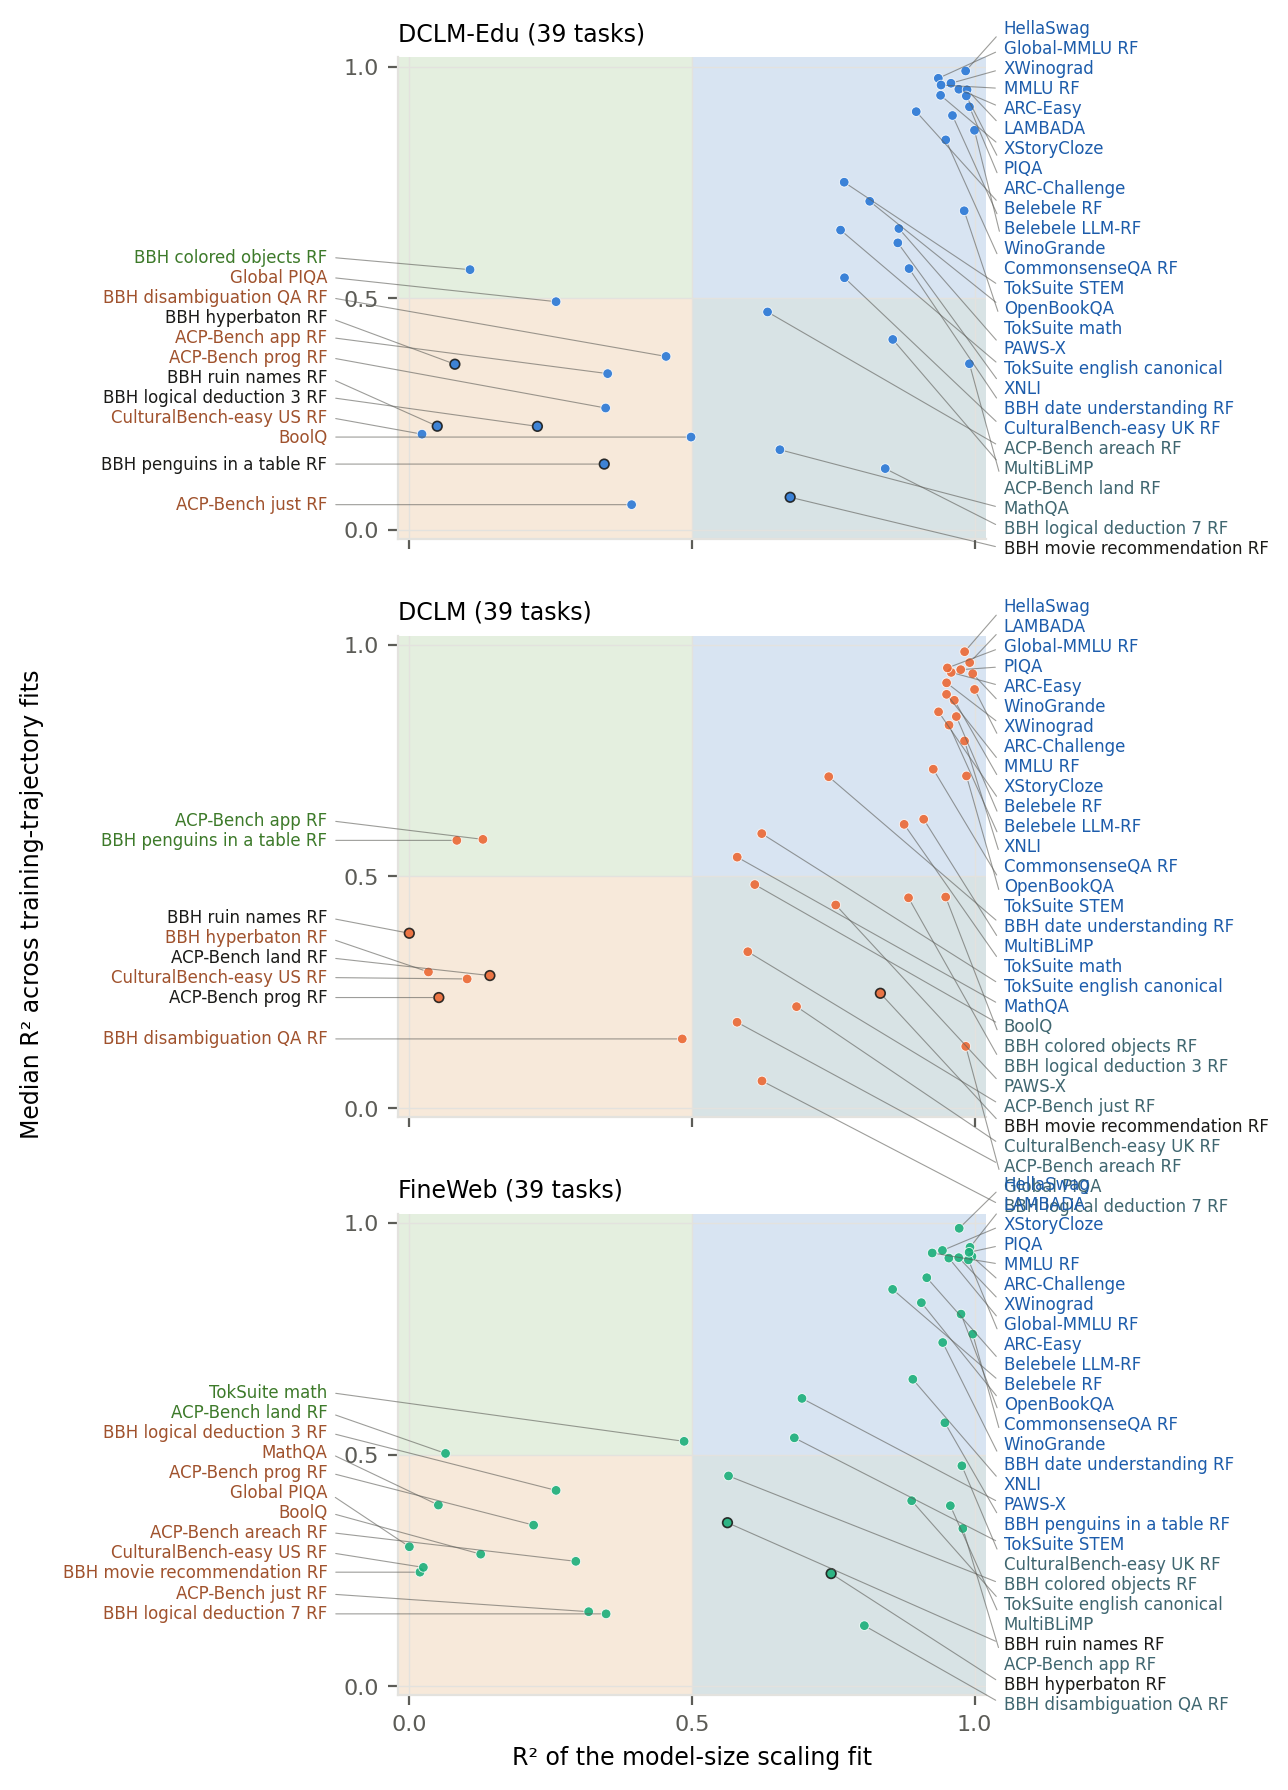
\includegraphics[width=\textwidth,height=0.8\textheight,keepaspectratio]{figures/app_rq13_english_scaling_regimes_l1_accuracy_tagged.png}
% source: src/signal-and-noise/analysis/rq13_english_only/pretraining/predictivity/english_only_scaling_regimes_l1_accuracy_tagged_paper.png
\caption{\textbf{The well-known English benchmarks are the predictable ones, and the popular tasks that drop out stay at chance rather than scale badly.} ARC-Challenge, ARC-Easy, HellaSwag, LAMBADA, OpenBookQA, Belebele RF, CommonsenseQA RF, Global-MMLU RF, MMLU RF, XNLI, XStoryCloze and XWinograd are predictable across both size and training in all three corpora. Belebele, CommonsenseQA, Global-MMLU, MMLU and TruthfulQA (mc2) never pass the above-chance filter in their original format, and Global PIQA is the one above chance that does not scale. The bottom row of Figure~\ref{fig:app_rq13_english_scaling_regimes_l1_accuracy}, one panel per English corpus ($K$ = 1), with every task named beside its panel, on the left when the $R^2$ of its model-size fit is below 0.5 and on the right otherwise. A name takes the colour of its regime (blue predictable across both, green during training only, slate across size only, brown weak in both, black declines with size). The 74 English accuracy tasks that the filter removes have no point.}
\label{fig:app_rq13_english_scaling_regimes_l1_accuracy_tagged}
\end{figure*}
